\documentclass{article}
\usepackage[
top    = 2.75cm,
bottom = 2.50cm,
left   = 3.00cm,
right  = 2.50cm]{geometry}
\usepackage{hyperref}
\usepackage{cite}
\usepackage{setspace}
\usepackage{algorithm}
\usepackage{graphicx}
\graphicspath{ {./images/} }
\title{\vspace{-2.0cm} A Generalizable Framework for Automated Cloud Configuration Selection \\ \vspace{0.5cm} \large Supervisors: Adam Barker \& Yuhui Lin}
\date{2019-06-06}
\author{Jack Briggs - 140011358 \\ MSc Data-Intensive Analysis}
\doublespacing
\begin{document}
\maketitle
\newpage
\section*{Abstract}
Outline of the project using at most 250 words
\newpage
\section*{Declaration}
I declare that the material submitted for assessment
is my own work except where credit is explicitly
given to others by citation or acknowledgement. This
work was performed during the current academic year
except where otherwise stated.
The main text of this project report is NN,NNN* words
long, including project specification and plan.
In submitting this project report to the University of St
Andrews, I give permission for it to be made
available for use in accordance with the regulations of the University Library. I also give permission for the title and abstract to be published and for copies of the report to be made and supplied at cost to any bona fide library or research worker, and to be made available on the World Wide Web. I retain the copyright in this work.
\newpage
\tableofcontents
\listoffigures
\newpage
\section{Introduction}
\textbf{Describe the problem you set out to solve and the extent
of your success in solving it. You should include the aims
and objectives of the project in order of importance and
try to outline key aspects of your project for the reader to look for in the rest of your report.}
\subsection{Background}
%Describe the use of cloud servers
%Describe how picking cloud configurations are difficult
%Describe how an automated tool can help

\subsection{Aims and Objectives}
%Safe spot
Algorithm
%Generalizable tool to use a given objective fit measure to find the optimal cloud configuration
%Extensions
Multiple cloud providers
Latency/response tests from a separate machine
Concurrent jobs to reduce search time
\subsection{Contributions}
% Made a good framework for automated cloud testing
% Experimentally shown how Bayesian Optimization's effectiveness changes based on search space and parallelisation (reduced search space increases effectiveness, parallelisation reduces search time but also effectiveness without stricter stopping conditions)

\subsection{Dissertation Overview}
% Context summary, describing previous work and availabe tools that will be used.
% Formalizng the requirements specification
% Describing Software engineering process and the design
% Explaining and describing the final implementation
% Evaluate and critically discuss it.
% Conclude by discussing future extensions and ways to make it more consumer-facing


\section{Literature Survey}
\textbf{Surveying the context, the background literature and any
recent work with similar aims. The context survey
describes the work already done in this area, either as
described in textbooks, research papers, or in publicly
available software. You may also describe potentially
useful tools and technologies here but do not go into
project-specific decisions.} \\

% Existing work (Cherrypick (BO), PARIS)
% Technical background (Terraform, Spearmint)

%First ways of actually evaluating the performance of a black box app
%Then describing previous configuration testers 
	% How Cherrypick was extremely effective and used an open-source BO tool spearmint that will be used
%Problem of making it work across multiple providers, leading to modern Infrastructure as code developments


\section{Requirements Specification}
\textbf{Capturing the properties the software solution must have
in the form of requirements specification. You may wish
to specify different types of requirements and given them
priorities if applicable.}

Previous solutions to the problem of automated cloud configuration selection have focused on specific use-cases or application types, and have not provided a functional implementation.  Our design should be generalisable to any form of application deployed on the cloud, and should be able to recreate previous solutions. This paper should also come with an associated implementation, which can at least perform a Bayesian Optimization-based search for a given docker container containing a batch job or benchmark.


\subsection{Use-case}
\section{Design}
\textbf{Indicating the structure of the system, with particular
focus on main ideas of the design, unusual design
features, etc. \\}
\begin{figure}[!ht]
  \caption{A diagram of the design.}
  \label{fig:design}
  \centering
   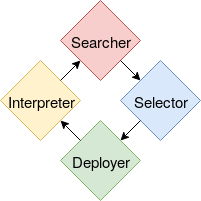
\includegraphics[scale=0.8]{Design}
\end{figure}

Optimisation is the process of minimising or maximising the value of some objective function by adjusting its input variables or parameters. Any optimisation algorithm begin with an initial guess of these variables and iterate through improved estimates until they terminate, hopefully providing an estimated solution. \cite{Nocedal2006} In the generalized case, the optimisation method and objective function are both unknown, but we know that our objective function will always involve selecting some cloud configuration based on the inputs, deploying some application onto this configuration, and interpreting its performance to give some objective measure.

This process can be broken down into four components: A Searcher, which runs the optimisation algorithm, testing out various inputs in an attempt to maximise or minimise the objective function; a Selector, which interprets the inputs to determine what cloud configuration is being tested; a Deployer, which deploys the application onto this cloud configuration and returns any required logs from it; and an Interpreter, which takes these logs to calculate the objective measure which is returned to the Searcher as the returned value for the objective function. A diagram of this breakdown is shown in figure \ref{fig:design}.

It is assumed that in the vast majority of cases, the user would provide their own Interpreter and Selector, that in some cases they must provide their own Deployer, and that only in rare cases would the user be required to provide their own Searcher. This is because optimization algorithms can be applied to any deployments, with only small modifications necessary in rare cases for specific cases. Deployments can often be contained within Docker containers, and aside from occasional setup, for example in multi-node clusters, a Deployer which provisions a given configuration from a given provider, and then deploys and attaches to a user-provided docker image to collect its logs will be sufficient. Interpreters and Selectors, on the other hand, are very dependent on the form these logs will take, and the form the search space will take, and are extremely hard to generalise. For this reason, the modular design of our solution should make it simple for any component to be supplied or replaced by the user. 

For each component

\subsection{Searcher}
The Searcher component performs an optimisation algorithm, such as Bayesian optimization, coordinate descent, random search, or exhaustive search, and drives the optimization process by iterating through potential input variables. For each set of these inputs, it take a sample from a single 'job,' and run through a single loop of the other three components. The constraints for these input variables must be specified, by describing their type (integer, float, categorical) and limits. A description of how to model cloud configurations into a set of variables is done in the Selector section.

\subsubsection{Example - Grid/Exhaustive search}
In an exhaustive search, every possible combination of the inputs is sampled, giving a complete analysis of the entire search space. This obviously takes many samples, $n * \prod_{i=1}^{j} x_{i}$ where $x_{i}$ is the number of options for the \textit{i}th of J variables, and n is the number of samples taken from each configuration. This results in a large or even infinite search cost and time, but is almost certain to return the optimal result, depending on the amount of randomness involved in sampling. A grid search is similar, but rather than sampling at every possible option within the search space, samples at regular intervals within it to reduce the number of samples taken. A coarser grid search results in a quicker, cheaper search, but a less confident prediction.

\subsubsection{Example - Bayesian Optimization}
% Variable for CPU can actually be an integer, which is done to the power of 2.

\subsection{Selector}
The Selector interprets the variables provided by the Searcher component into the form of a cloud configuration that can be deployed. Cloud configurations have a number of variables that can describe them, such as vCPU number, Memory amount, number of instances, instance category, machine type, and cloud provider. The selector must use whatever combination of these is provided and find either the exact or most similar cloud configuration available, passing this information on to the Deployer.

\subsubsection{Example - Exact Match}
\subsubsection{Example - Closest Match}
% This would require a record to be kept of previously tested instances so as not to repeat similar instances multiple times. In cases of significant noise it may be beneficial to test multiple times, so can limit this to 3.
% Driver function reads the files to make a configuration dictionary to be passed to other functons. It reads the variables into this and well as loads the functions specified in the variable file. At the end of each job, this configuration dictionary is saved as a json file for later analysis, as well as being appended to a json file that incorporates all the logs from any previous jobs performed by the function. (This file should be regularly backed up, probably into separate smaller files, as otherwise an error can throw away lots of data)
\subsection{Deployer}
The Deployer deploys the user-provided application, batch job, or benchmark onto the selected cloud configuration, and collect any necessary analysis from it. Typically this will involve provisioning the necessary machines from the given provider, followed by deploying the given application onto these machines, and either collecting logs from them or from a networked instance or cluster. 

\subsubsection{Example - VM Provisioner}
The deployer should be capable of handling any response from the selector, and must work with multiple providers. This can be simplified using Infrastructure as code (IaC) tools such as Terraform or Chef.
\subsubsection{Example - Docker Deployer}
\paragraph{vBench}
\paragraph{Cloudsuite3}
\paragraph{Sysbench}
\subsubsection{Example - Ping server}
\subsubsection{Example - Fake Deploy/Old Deploy}

%Also fake deploy for debugging, or old_deploy for using already gathered results

\subsection{Interpreter}
% Interpreters were made for all those listed above (vBench, cloudsuite3 media streaming, sysbench

The Interpreter must interpret whatever information is returned by the Deployer, along with the cost of the cloud configuration, in order to give the searcher an objective measure for the sampled cloud configuration. It is this returned value which will be minimized or maximized. By its nature, the interpreter will most likely be unique for a given application.

\section{Implementation}
\textbf{How the implementation was done and tested, with
particular focus on important / novel algorithms and/or
data structures, unusual implementation decisions, novel
user interface features, etc.}
\subsection{Searcher}
For the sake of generalizability, the available implementation of spearmint was found to be outdated and incompatible with the latest versions of various python modules planned to be used in later steps. 
Because of this, spearmint was first updated to be compatible with Python 3 and newer versions of its dependencies such as Google Protocol Buffers. This implementation of spearmint has been made available.\footnote{https://github.com/briggsby/spearmint3}

\subsection{Selector}
% Why we only evaluated exact match. Problems with closest match. If there are architectural problems the user may want to avoid certain instance types. A selector that uses an API to retreive available instance models may be useful.

\subsection{Interpreter}
% We used very simple metrics of dividing scores (which were various measures of number of users/rate of transcoding/rate of response/number of operations) by the hourly price. This is not likely to correspond to a real metric used in business, where even a small advantage over a competitor can lead to a dramatic uptake in users, but was effective for evaluation.
\section{Evaluation}
\textbf{You should evaluate your own work with respect to your original objectives. You should also critically evaluate your work with respect to related work done by others. You should compare and contrast the project to similar work in the public domain, for example as written about in published papers, or as distributed in software available to you.}

To demonstrate the effectiveness of the implementation of our framework, we wanted to show that it could replicate the methods set out in the Cherrypick paper \cite{Alipourfard2017} by performing Bayesian Optimization to attempt to find an optimal configuration for a given deployment. We then wanted to use the same implementation to perform multiple exhaustive searches so that the results from Bayesian Optimization could be properly compared to the real average results. 

The deployment to be used was originally planned to be Cloudsuite3's media streaming benchmark, however this was found to be extremely variable and dependent entirely on network bandwidth, and so instead the vBench video transcoding benchmark was used. Our objective function measured an instance type's relative rate of transcoding of a single 5 second 1920x1080 video file, returning a score of 0 if the quality was below a given threshold, divided by the hourly price of that instance. Effectively, we maximised the rate of transcoding a unit of video length at a sufficient quality per hourly cost. 

For choosing the boundaries of the search space, we decided to reduce costs by using only machines ranging from 2 vCPUs to 8 vCPUs. This was also convenient as to use more powerful machines would have required requesting additional raised quotas from the providers used, and so would be less easily replicable. Using exact match, and as we wanted to show that the implementation worked with multiple providers, we could not rely on Google cloud platform's custom machine types and had to find some way to categorize possible variables. Rather than including memory as a variable, CPU instead was coded as a categorical variable (2, 4, or 8), along with machine category (General, Memory, CPU), each with a different amount of memory. Table \ref{tab:instance-types} show which machine types corresponded to each option. 

\begin{table}
\begin{tabular}{ |c||c|c|  }
 \hline
 & \multicolumn{2}{|c|}{Provider} \\
 \hline
 Machine Category & Amazon EC2 & Google Compute Engine \\
 \hline
 General& n1-standard & m5\\
 Memory & n1-highmem  & r5\\
 CPU    & n1-highcpu  & c5\\
 \hline
\end{tabular}
\caption{Machine types corresponding to different instance categories for the two providers}
\label{tab:instance-types}
\end{table}

For realistic situations, the search space could follow this same pattern, with the CPU variable extended, possibly instead as an integer between 1 and 6 which 2 is raised to the power of to determine vCPU number, as this covers many of the available CPU options.

The 18 machine types decided upon (3 vCPU numbers for 3 machine categories for the 2 providers) were stored in a single dataset for use with the 'Exact match' instance selector. The vBench deployer was used which utilized Terraform to provision a single instance of the given machine type, on which the remote docker api was used to deploy and collect logs from an docker image containing vBench. The vBench interpreter then isolated the vBench score from these logs, and divided it by the hourly cost of that machine type to return the final value.

Where not otherwise specified, statistical results are quoting the p-values returned from a Tukey's Honest Significant differences test to correct for multiple comparisons.

The results of the exhaustive search are shown in figures \ref{fig:vBench-scores} and \ref{fig:vBench-values}. The raw scores (time taken to transcode relative to the reference) show clear overlap between many possible configurations, and in general show a significant difference between 2 vCPUs and either 4 ($P < .001$) or 8 ($P < .001$) vCPUs, with a larger number of vCPUs increasing the score, but show less clear differences between 4 and 8 ($P = .066$), dependent on the provider and machine category, suggesting either diminishing returns or a limit of the benchmark to utilize all vCPU cores.
 
\begin{figure}
  \centering
   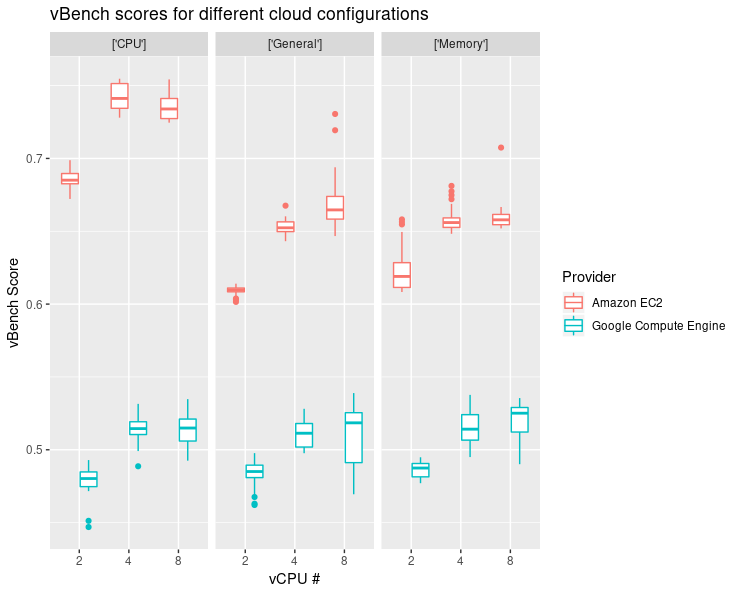
\includegraphics[scale=0.8]{vbench_scores}
   \caption{Distribution of vBench scores}
  \label{fig:vBench-scores}
\end{figure}
\begin{figure}
  \centering
   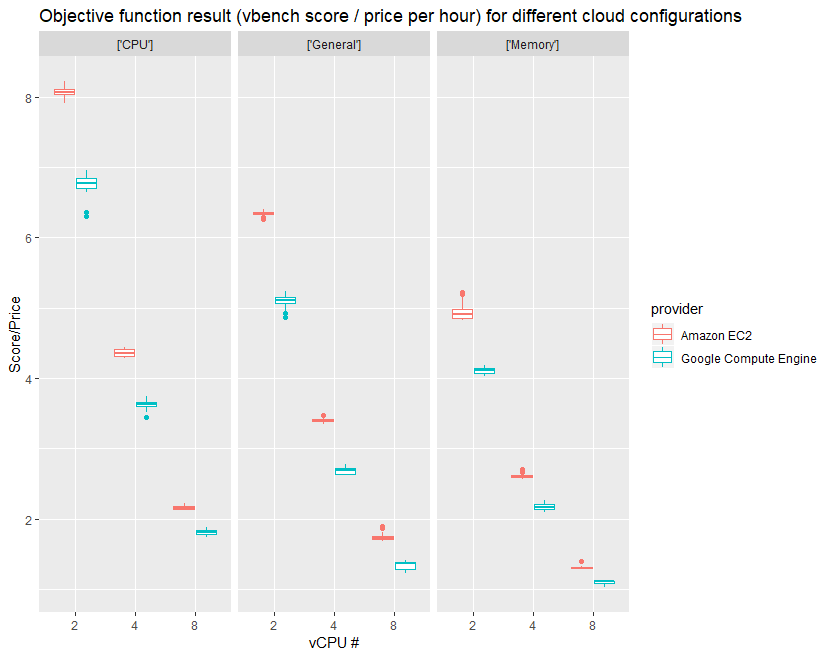
\includegraphics[scale=0.8]{vbench_values}
   \caption{Distribution of objective function values}
  \label{fig:vBench-values}
\end{figure}
\begin{figure}
  \centering
  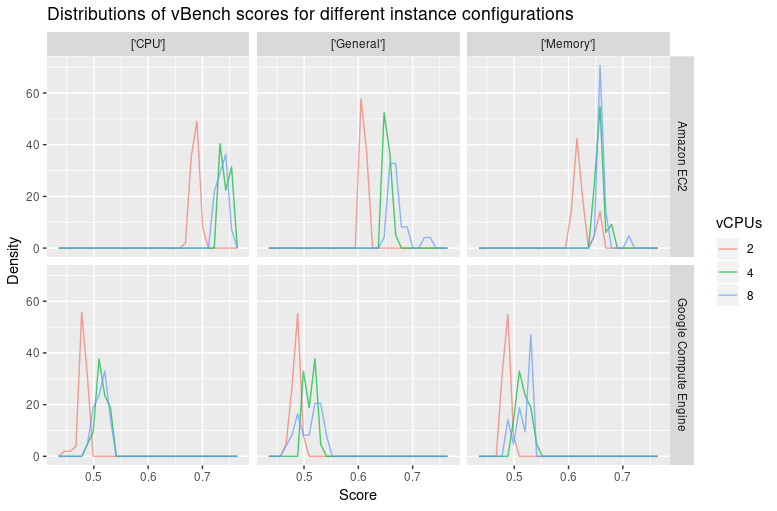
\includegraphics[scale=0.8]{vbench_dists}
  \caption{Distribution of vBench scores in frequency polygons}
  \label{fig:vBench-dists}
\end{figure}

However, once the scores are instead given relative to the machine's hourly costs, there is much less overlap. A clear optimal configuration can be seen in the c5.large machine type, if one is purely interested in getting the most video transcoding for a given cost. The c5.large machine was significantly better than the next best option, the n1-highcpu-2 ($P < .001$). Amazon EC2's  machine types consistently outperformed Google Compute Engine's equivalents of the same category and vCPU number at both raw score (Anova, $F = 32111.456, P < .001$) and value for money (Anova, $F = 22710.7, P < .001$). However, despite this general trend, the provider seemed to be the least important factor in determining the optimal configuration. For example, the n1-highcpu-2 still gave significantly better values than the m5.large ($P < .001$), or the c5.xlarge ($P < .001$) making it the second most cost-efficient option. 

\begin{figure}
  \caption{Optimal configurations found after convergence for Bayesian Optimization}
  \label{fig:bo-results}
  \centering
  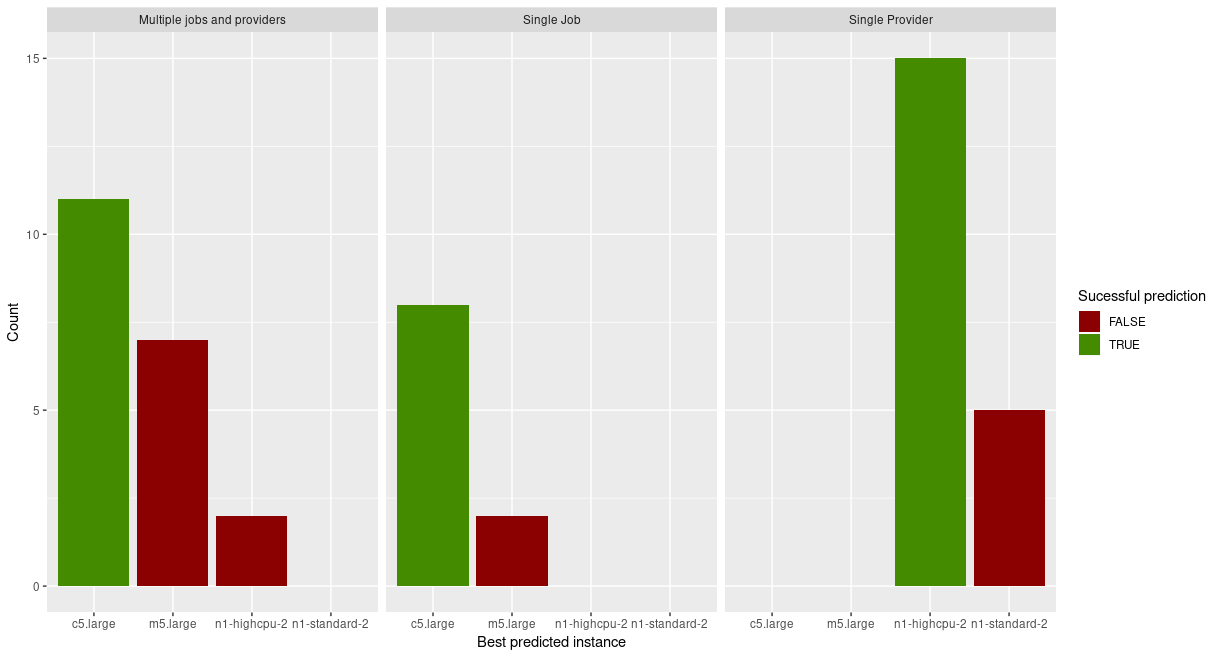
\includegraphics[scale=0.5]{bo_results}
\end{figure}
\begin{figure}
	\centering
	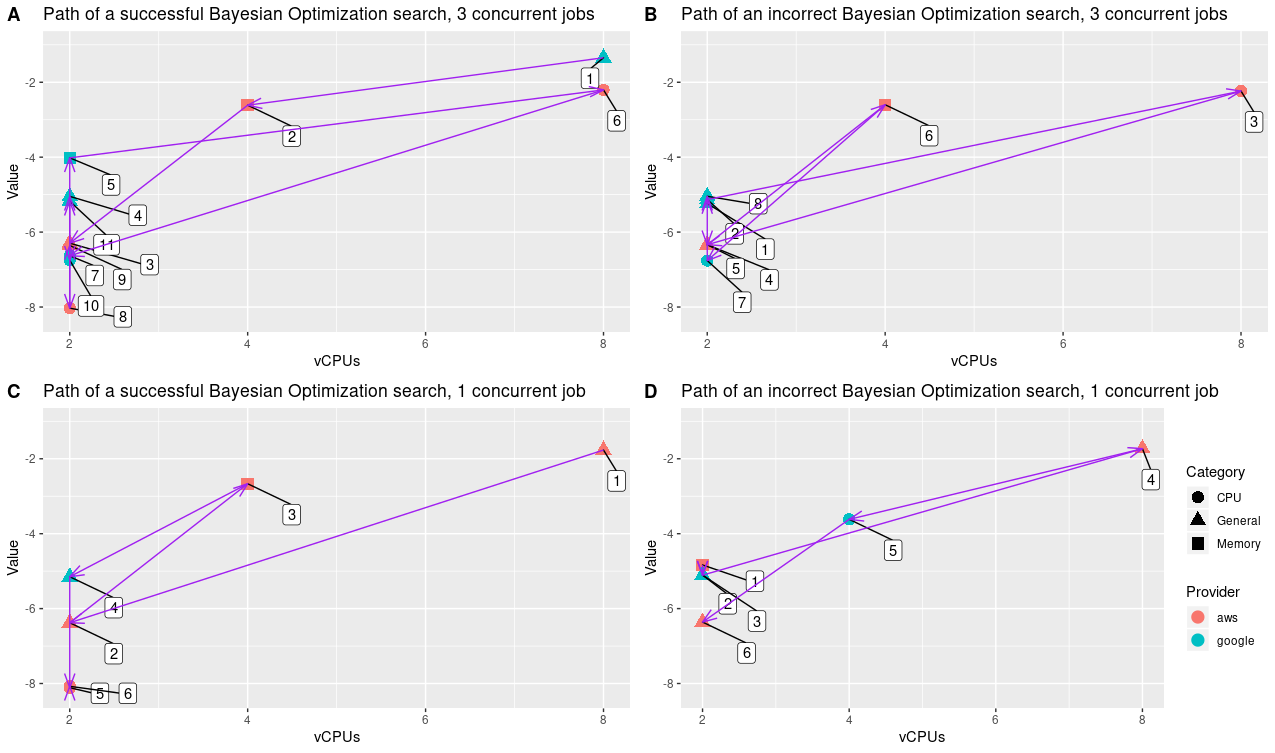
\includegraphics[scale=0.5]{paths}
	\caption{Paths of example Bayesian Optimization jobs}
	\label{fig:paths}
\end{figure}

With the exhaustive search complete, we then used a Spearmint based searcher to perform a Bayesian Optimization search, assuming low noise (-1 to 1) and using the same stopping conditions as used by default in the Cherrypick paper \cite{Alipourfard2017}, namely when the Expected improvement (EI) is less than 10\%, and at least 6 samples have been taken. We were able to successfully run this experiment with both multiple and single providers, as well as with both single jobs and multiple concurrent jobs. The results from these experiments are shown in figure \ref{fig:bo-results}, while examples of the job paths taken during them are shown in figure \ref{fig:paths}.

With only a single concurrent job running, we were able to replicate the previous results, with the correct optimal instance predicted in 8 out of 10 evaluations. It is interesting to note, however, that the incorrectly predicted instance in both failed cases was not the second but third best choice, resulting in a reduction in the score/cost value by ~21.3\%.

While running multiple concurrent jobs could dramatically decrease the search time, it did come at a cost to accuracy. With the same stopping conditions, a successful prediction was made only 12 out of 20 experiments (60\%). This suggests that multiple concurrent jobs is only a good choice when reducing search time is more important than reducing search cost, as more stringent stopping conditions should be used.  Unsurprisingly, reducing the search space to a single provider increased the likelihood of making correct predictions with multiple concurrent jobs, leading to 15 correct predictions out of 20 repeats (75\%).

Having performed evaluation on our implementation for a deployment of a simple docker container, effectively corresponding to running a single batch job or benchmark and interpreting the results, we then wanted to evaluate the same technique applied to an web-based application, which may be better evaluated through its responses to a client. For this a single 5-node Kubernetes cluster was set up for the same of sending repeated requests to the evaluated deployment, as described for the 'Pingserver' deployer and interpreter. This experiment is much more intensive to perform exhaustive search for, as it would require separate pinging clusters to be set up for every sample. The mean response time for requests of a normally distributed load was divided by the hourly cost of the instance to give maximised value. From the samples taken during 10 repetitions of this experiment, it seemed that there were no significant difference between the two optimal configurations of c5.large and m5.large ($\Delta \bar{x}=0.0001, P \approx 1.000$), which the predictions correctly converged upon in all cases.

\subsection{Related Work}


\section{Critical discussion}
\textbf{You should evaluate your own work with respect to your
original objectives. You should also critically evaluate
your work with respect to related work done by others.
You should compare and contrast the project to similar
work in the public domain, for example as written about
in published papers, or as distributed in software available to you. }

As mentioned, the evaluation above likely does not correspond to comparisons with which to base real deployment decisions on. In reality, a small increase in transcoding speed may lead to a far greater increase in customer uptake, rather than the effectively 1:1 ratio between price and transcoding speed assumed in the experiment. However, the evaluation shows that the methodology works very well with a given objective score measure, and it would be trivial for a new objective function to be implemented with a different relationship between the score, price, and 'value' of a given configuration.
\subsection{Future extensions}
% There is a really good space to try this with serverless computing, but cloud run is currently not supported with terraform making this more difficult.
% If time allows could write a quick bash script to try this.
% When limited to google the search space becomes much better suited for Bayesian Optimization because of the non-categorical choices with vCPU and Memory amounts
\section{Conclusions}
\textbf{You should summarise your project, emphasising your
key achievements and significant drawbacks to your
work, and discuss future directions your work could be
taken in.}
\newpage
\bibliographystyle{ieeetr}
\bibliography{Dissertation}
\newpage
\section*{Appendices}
\subsection*{Testing Summary}
\subsection*{User Manual}
\end{document}